
%%% Local Variables:
%%% TeX-command-extra-options: "-shell-escape"
%%% mode: latex
%%% TeX-master: t
%%% End:
\documentclass{beamer}
\usepackage{caption}
\usepackage{minted}
\usepackage[labelformat=simple]{subcaption}

\usetheme{Boadilla}
\title{Lecture 2}
%\subtitle{in Racket}
%\author{Peter Campora}
%\institute{ULL}
%\date{\today}

%This lectures introduces Dr. Racket and the wrong way to program
\begin{document}
\begin{frame}
\titlepage
\end{frame}

\begin{frame}
  \frametitle{Dr. Racket}
  \begin{columns}
    \column{0.45\textwidth}
    I encourage the use of Dr. Racket:
    \begin{itemize}
    \item<1-> The definitions window (top) is for writing programs
    \item<2-> The interactions window (bottom) is for interaction
    \item<3-> Let me demonstrate 
    \end{itemize}
    \column{0.45\textwidth}
    \begin{figure}
      \centering 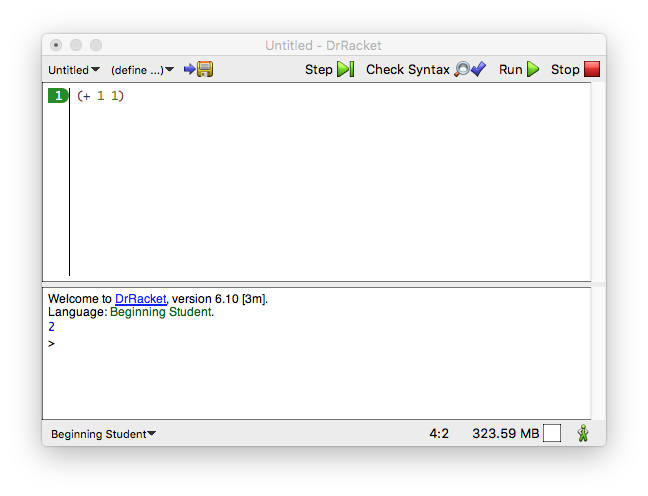
\includegraphics[width=0.9\textwidth]{images/drracket-plain.png}
    \end{figure}
  \end{columns}
\end{frame}

\begin{frame}
  \frametitle{Relevant XKCDs}
  \begin{figure}
    \centering 
\includegraphics[width=0.8\textwidth]{images/lisp_cycles.png}
  \end{figure}    
  % 
  \begin{figure}
    \centering 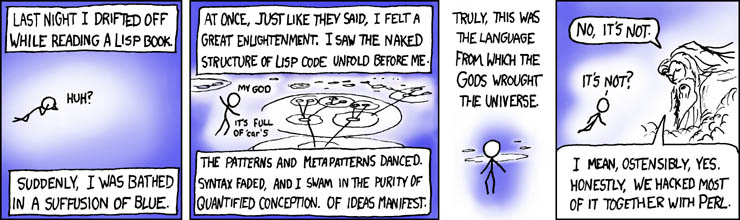
\includegraphics[width=0.8\textwidth]{images/lisp.jpg}
  \end{figure}    
\end{frame}

% \defverbatim[colored]\lstR{
% \begin{minted}{Scheme}
% ;;Number -> Number
% (define (square x) (* x x))

% ;;Number List -> Number List
% (define (sum-of-squares lst)
%   (sum (map square lst))         
% \end{minted}
% }

\defverbatim[colored]\syntaxOne{
\begin{minted}{Scheme} 
    (f 1)  
\end{minted}
}

\defverbatim[colored]\syntaxTwo{
\begin{minted}{Scheme} 
    (+ 1 2)
\end{minted}
}

\defverbatim[colored]\syntaxThree{
\begin{minted}{Scheme} 
    (+ 1 (* 2 3))
\end{minted}
}

\defverbatim[colored]\syntaxFour{
\begin{minted}{Scheme} 
    (define (double x) (* x 2))
\end{minted}
}

\begin{frame}
  \frametitle{Syntax Primer}
  Functional Programming is about \emph{functions}
  \begin{itemize}
  \item<1-> To call a function f, with argument 1 we write: \syntaxOne
  \item<2-> Instead of 1+2 we write: \syntaxTwo
  \item<3-> There is no operator precedence. 1 + 2*3 becomes: \syntaxThree
  \item<4-> To define a function that doubles numbers: \syntaxFour
    
  \end{itemize}
\end{frame}

\end{document}